

\chapter{خودکار سازی}

ایجاد پروژه آخرین کاری است که در یک پروژه نرم‌افزاری انجام می‌شود. در این  فاز
تمام برنامه‌های نوشته شده توسط توسعه دهندگان سیستم ترجمه شده و یک برنامه اجرایی
ایجاد می‌شود. کارهایی که در این فاز از پروژه انجام می‌شوند عبارت‌اند از:

\begin{itemize}
  \item ترجمه برنامه‌ها به برنامه‌های اجرایی
  \item ایجاد بسته‌های نرم‌افزاری مبتنی بر برنامه‌های اجرایی
  \item ارزیابی و بررسی کیفیت محصول
  \item ایجاد قابلیت انتقال به روی سیستم‌های متفاوت
  \item ایجاد مستند و راهنما
\end{itemize}

گرچه ممکن است که فرآیند ساخت از یک پروژه به پروژه دیگر متفاوت باشد اما این
فرآیند به صورت مشابه و یکنواخت در تمام آنها اجرا می‌شود. برای نمونه گرچه در
پروژه‌های که از زبانهای مفسری مانند \lr{PHP} استفاده شده باشد ترجمه برنامه به
برنامه‌های اجرایی هرگز انجام نمی‌شود اما مراحل دیگر ساخت پروژه همچنان پا برجا
خواهد بود.

از آنجا که این کار تنها توسط توسعه دهندگان سیستم قابل اجرا و در تمام
پروژه‌ها مورد نیاز است، دور از تصور نیست که این فرآیند به صورت خودکار و توسط یک
ماشین قابل اجرا باشد. خودکار سازی در اینجا نیز به این نکته اشاره دارد. با
استفاده از روش‌های خودکار ساخت پروژه نه تنها می‌توان از میزان هزینه‌ها مانند
زمان و نیروی انسانی کاست بلکه می‌توان به کیفیت کار انجام شده نیز افزود.

ساخت خودکار یک پروژه نرم‌افزاری عبارت است از یک نپشته\LTRfootnote{Script}،
برنامه و یا هر سیستم دیگری که مراحل ساخت یک پروژه را به صورت خودکار و بدون دخالت
کاربر انجام دهد.
    
% History

ابتدایی ترین تلاش‌ها برای خودکار سازی فرآیند ساخت توسط توسعه دهندگان سیستم‌ها
بود. توسعه دهندگان با استفاده از برنامه‌ها و نپشته‌ها مترجم‌ها و پیوندگرها را با
استفاده از دستورهای خط فرمان فراخوانی و با استفاده از آن برنامه‌های
اجرایی را ایجاد می‌کردند. برای نمونه با استفاده از نپشته زیر که در سکوی لینوکس
قابل اجرا است می‌توان تمام پرونده‌های ایجاد شده در یک پروژه سی را ترجمه کرده و
یک برنامه اجرایی ایجاد کرد.

\begin{latin}
\lstset{language=BASH}  
\begin{lstlisting}[frame=single] 
#!/bin/bash
DIR="$1"
OUT="$2"
[ "$DIR" == "" ] && DIR="."
fileArray=($(find -name "*.c"))

#Compile and creat object file
for file in ${fileArray[*]}
do
	g++ -Wall -O $file -o ${file}.o
done

#Link all objrct file
for file in ${fileArray[*]}
do
	g++ ${file}.o $OUT
done

\end{lstlisting}
\end{latin}

با استفاده از این نپشته تمام پرونده‌های \lr{*.c} در یک مسیر با استفاده از مترجم
\lr{g++} ترجمه شده و با استفاده از پیوندگر\LTRfootnote{Linker} یک برنامه اجرای
ایجاد می‌شود.
گرچه این نپشته بسیار ساده است اما به عنوان ابتدایی ترین سیستم‌های خودکارسازی
فرآیند ساخت مورد استفاده قرار می‌گرفته است.

استفاده از دستورهای خط فرمان و ترجمه تک تک برنامه‌های نوشته شده و درنهایت ایجاد
یک برنامه اجرایی با استفاده از یک پیوندگر ساده است. اما زمانی که نیاز به ترجمه
پروژه‌های بزرگ که از قطعه‌های متفاوتی ایجاد شده‌اند و بین آنها وابستگی از پیش
تعریف شده‌ای وجود دارد استفاده از این روش‌های ساده مناسب نیست.

تلاش بعدی توسعه دهندگان سیستم‌های نرم‌افزاری منجر به ایجاد برنامه‌ها و زبانهای
جدید برای خودکار سازی فرآیند ساخت شد. از این میان می‌توان به زبان \lr{Make}
اشاره کرد. این زبان خودکار سازی را می‌توان به عنوان یک جایگزین مناسب برای
نپشته‌های ابتدایی در نظر گرفت. نپشته‌های مورد استفاده در این ابزار امکان نوشتن
وظایف متفاوت مانند ترجمه و پیوند به صورت متوالی  وجود دارد. نسخه‌های ایجاد شده
توسط گروه \lr{GNU} نه تنها توانایی یاد شده را فراهم کرده است بلکه توانایی ساخت
موازی، توزیع شده و یا ایجاد بر اساس وابستگی‌ها نیز فراهم شده است.

اما این تنها آغاز راه بود و فرآیند ساخت به سرعت پیچیده شد. در ابتدا فرآیند ساخت
تنها به ترجمه و پیوند برنامه‌ها توجه داشت. امروزه فرآیند ساخت انقدر پیچده شده
است که نه تنها مترجم‌ و پیوندگرها مورد استفاده قرار می‌گیرد بلکه از سیستم‌های
متفاوت دیگر مانند مستندگر، کنترل نسخه، برنامه‌های ارزیابی و بسیاری دیگر مورد
استفاده قرار می‌گیرد. 

در حال حاضر فرآیند ایجاد شامل وظایف متفاوتی چه قبل از ترجمه و چه بعد از ترجمه
می‌شود. فرآيند ساخت آن چنان پیشرفت کرده است که امروزه بر فرآیند توسعه سیستم‌های
نرم‌افزاری تاثیر گذاشته و منجر به ایجاد متدلوژی‌های جدیدی شده است.

% TODO : maso 1391 : روش‌های CI و ایجاد توزیع شده را باید بررسی کنم

% New breed of solutions

امروزه گونه‌های جدید ابزارهای خودکار سازی فرآیند ساخت امکانات بسیار متفاوت و
مناسبی را ارائه می‌کنند.
این ابزارها به صورت‌های متفاوتی چون نرم‌افزارهای متن باز و یا تجاری ارائه
می‌شوند.
در بسیاری از این ابزارها تمرکز به روی اجرای نپشته‌های ایجادگر است در حالی که
گونه‌های دیگر با توجه به کارهای مورد نیاز پیش و پس از فرآیند ساخت تلاش دارند که
ابزارهای مناسب برای ساده سازی این فرآیند را ارائه کنند. هدف اصلی در ساده سازی
فرآیند ساخت فراخوانی راحت مترجم‌ها، پیونگرهای و دیگر ابزارهای مورد نیاز در
فرآیند ساخت است.
استفاده از این ابزارها در فرآیندهای توسعه مبتنی بر ساخت\LTRfootnote{Continous
Integeration} بسیار اساسی است تا جایی که توسعه سیستم بدون این سیستم‌ها غیر ممکن
می شود.


% Advanced build automation

ابزارهای مدرن ساخت از پیشکارهای\LTRfootnote{Agent} دور برای ایجاد پروژه به صورت
توزیع شده استفاده می‌کنند. واژه ساخت توزیع شده\LTRfootnote{Distributed
builds} به معنی فراخوانی مترجم و پیوندگر به صورت توزیع شده به روی ماشین‌های
متفاوت است که منجر به افزایش سرعت فرآیند ساخت می‌شود.
این واژه به صورت معمول با واژه محاسبات توزیع شد\LTRfootnote{Distributed
Processing} به اشتباه گرفته می‌شود.

% Distributed processing means that each step in a process or workflow can be sent
% to a different machine for execution. For example, a post step to the build may
% require the execution of multiple test scripts on multiple machines. Distributed
% processing can send the different test scripts to different machines.
% Distributed processing is not distributed builds. Distributed processing cannot
% take a make, ant or maven script, break it up and send it to different machines
% for compiling and linking.
% 
% The distributed build process must have the machine intelligence to understand
% the source code dependencies in order to send the different compile and link
% steps to different machines. A build automation solution must be able to manage
% these dependencies in order to perform distributed builds. Some build tools can
% discover these relationships programmatically (Rational ClearMake
% distributed[1], Electric Cloud ElectricAccelerator[2]), while others depend on
% user-configured dependencies (Platform LSF lsmake[3])
% 
% Build automation that can sort out source code dependency relationships can also
% be configured to run the compile and link activities in a parallelized mode.
% This means that the compiler and linkers can be called in multi-threaded mode
% using a machine that is configured with more than one core.
% 
% Not all build automation tools can perform distributed builds. Most only provide
% distributed processing support. In addition, most solutions that do support
% distributed builds can only handle C or C++. Build automation solutions that
% support distributed processing are often make based and many do not support
% Maven or Ant.
% 
% An example of a distributed build solution is Xoreax's IncrediBuild[4] for the
% Microsoft Visual Studio platform or the open-source CMake[5]. These may require
% particular configurations of a product environment so that it can run
% successfully on a distributed platform—library locations, environment variables,
% and so forth.

از سویی استفاده از پیشکارهای متفاوت با گونه‌های متفاوت امکان ایجاد یک سیستم
نرم‌افزاری مبتنی بر سکو‌های متفاوت را نیز امکان پذیر می‌سازد. پیشکارهایی که به
روی سکوی لینوکس\LTRfootnote{Linux} تعبیه شده‌اند سیستم نرم‌افزاری را برای این
سکو ترجمه و به برنامه اجرای تبدیل می‌کنند در حالی که پیشکارهای تعبیه شده به روی
سکوی ویندوز\LTRfootnote{Windows} کار مشابه‌ای را برای سیستم عامل ویندوز انجام
می‌دهند.

% Advantages

خودکارسازی فرآیند ایجاد، منافع زیادی برای گروه توسعه به دنبال دارد. به عنوان
نمونه برخی از این موارد عبارت‌اند از:

\begin{itemize}
  \item افزایش کیفیت محصولها
  \item تسریع در فرآیند ایجاد
  \item کاهش کارهای بیهوده
  \item کاهش اشتباه در فرآیند ساخت
  \item کاهش وابستگی به فرد
  \item نگهداری تاریحچه ساخت برای دنبال کرده ایرادها
  \item کاهش هزینه‌ها
\end{itemize}

% Types
%     On-Demand automation such as a user running a script at the command line
%     Scheduled automation such as a continuous integration server running a nightly build
%     Triggered automation such as a continuous integration server running a build on every commit to a version control system.
% Requirements of a build system
% 
% Basic requirements:
% 
%     Frequent or overnight builds to catch problems early.[7][8][9]
%     Support for Source Code Dependency Management
%     Incremental build processing
%     Reporting that traces source to binary matching
%     Build acceleration
%     Extraction and reporting on build compile and link usage
% 
% Optional requirements:[10]
% 
%     Generate release notes and other documentation such as help pages
%     Build status reporting
%     Test pass or fail reporting
%     Summary of the features added/modified/deleted with each new build

در تمام فرآیندهای ساخت ایجاد مستند تکنیکی و کاربری یکی از مراحل ایجاد بوده و
بدون آن فرآیند ایجاد نرم‌افزار ناقض خواهد بود. در این گفتار ابزارهای خودکار سازی
فرآیند ساخت معرفی شده و تنظیم‌های مورد نیاز برای ایجاد مستند تکنیکی در آنها
تشریج می‌شود.

نکته‌ای که باید در این گفتار به آن توجه داشت این است که، همواره فرض بر این است
که در فرآیند توسعه از استانداردهای تعریف شده در این کتاب استفاده شده است. در غیر
این صورت مراحل و تنظیم‌های مورد نیاز کمی متفاوت خواهد بود.




\section{مدیریت بسته کلاه قرمز}


% در این قسمت باید در مورد این سیستم مدیریت بسته به صورت کامل بحث شود
\lr{RPM} یا مدیریت بسته کلاه قرمز\LTRfootnote{\Gls{red hat package manager}} یک
مجموعه ابزار نرم‌افزاری برای ایجاد و نصب و راه اندازی سیستم‌های نرم‌افزاری است. می‌توان
گفت که پیشینه \lr{RPM} به صورت جدایی ناپذیری با پیشینه سیستم عامل لینوکس در هم
آمیخته است، از این رو بررسی پیشینه‌ لینوکس مفید است. لینوکس یک پیاده سازی کامل
از سیستم‌های عمل شبیه \lr{Unix} است که مانند یک طوفان دنیای محاسبات رایانه‌ای را
درنبردید.

هم زمان با توسعه و گسترش یافتن لینوکس، رایانه‌های شخصی تولید شده مبتنی بر
فن‌آوری \lr{Intel}، که تا پیش از آن اسیر سیستم ترسناک و سیری ناپذیر ویندوز بوند،
به رایانه‌های کاملا چندکاره\LTRfootnote{Fully Multitasking}، با قابلیت استفاده
از شبکه و ایستگاهای کاری شخصی تبدیل شدند. تمام این تعییرها در سخت‌افزارها و
رایانه‌ها به دلیل زمان زیاد مورد استفاده در پردازشها و نیاز شدید استفاده از شبکه
بود.

برای به کار بردن بسیاری از سخت افزارها، شرکت‌های تولید کنند لوح‌های فشرده حاوی
سیستم‌عامل لینوکس و نرم افزارهای مورد نیاز آن را روانه بازار می‌کنند در حالی که
بسیاری از این نرم‌افزارها در شبکه جهانی قابل دسترس هستند.
سرهم بندی کردن نرم‌افزارهای مورد نیاز در سیستم‌عامل لینوکس بر اساس توزیع مورد
استفاده آن متفاوت است اما انچه که مهم است این است که عبارت \'پول هرچه را بدهی
آن را داری\' در اینجا دیگر صادق نیست.

یکی از توزیع‌های لینوکس که نام منحصر به فرد لینوکس کلاه قرمز\LTRfootnote{Red
Hat Linux} را یدک می‌کشید که توسط یک شرکت هم نام با آن توسعه می‌یافت. این توزیع
از سیستم‌عامل لینوکس کمی با دیگر توزیع‌های لینوکس موجود متفاوت بود. یکی از
مشکل‌ترین کارهای کاربران لینوکس تعیین این بود که کدام قسمت از نرم‌افزارهای موجود
در یک توزیع خاص از این سیستم‌عامل باید نصب و مورد استفاده قرار گیرد. در بسیاری
از توزیع‌های لینوکس انتخاب نرم‌افزارهای مورد نیاز برای نصب با استفاده از منوهایی
انجام می‌شد که استفاده از آن بسیار راحت بود و لینوکس کلاه قرمز نیز از این قاعده
مستثنا نبود.

اما تفاوت اصلی این توزیع با دیگر توزیع‌های لینوکس در این بود که سازندگان آن تلاش
داشتند که کاربران برای نصب یک بسته و یا نرم‌افزار کاری بیشتر از انتخاب بسته و یا
نرم‌افزار را انجام ندهند. با این وجود سیستم‌های تجاری یونیکس از سیستمی مشابه با
این نیاز استفاه می‌کرند که سیستم مدیریت بسته\LTRfootnote{Package Manger} نام
داشت. در همین راستا بسیاری از گروها در توزیع‌های متفاوت لینوکس تلاش کردند که
سیستم‌های مشابه‌ای را برای مدیریت بسته‌ها و نرم‌افزارهای ارائه دهند که هیچ کدام
به گستردگی \lr{RPM} نبود.

با گذر زمان توزیع کلاه قرمز لینوکس محبوب‌ترین توزیع لینوکس شد که امروز در دسترس
بسیاری از کاربران است. مهم‌ترین عامل موفقیت این توزیع از سیستم‌عامل لینوکس را
می‌توان \lr{RPM} معرفی کرد. گرچه در اینجا یک توصیف کوتا از این سیستم مدیریت بسته
اورده شده است اما با این وجود می‌توان کاربرد فوق تصور این روش در مدیریت
نرم‌افزارها را به سادگی حس کرد.

اما در دنیای نرم‌افزارهای رایگان یک اصل اولیه وجود دارد که عبارت است: زمانی که
یک سیستم نرم‌افزاری رایگان راهکار مناسب‌تری را ارائه می‌دهد، از آن استفاده کن.
سیستم مدیریتی \lr{RPM} نیز از این قائده مستثنا نیست. از این رو توانایی‌های
موجود در این سیستم به سرعت توجه بسیاری از کاربران و توسعه دهندگان نرم‌افزارهای
رایگان را به خود جلب کرد.

در حال حاضر علاوه بر گروه‌هایی که نرم‌افزارهای رایگان  را توسعه می‌دهند، بسیاری
از شرکت‌ها وجود دارند که محصولات تجاری خود را نیز بر اساس \lr{RPM} روانه بازار
می‌کنند. این شرکت‌ها نه تنها به این نکته دست یافته‌اند که با استفاده از این
سیستم مدیریت نرم‌افزار محصولات آنها راحت‌تر در دسترس مشتریان قرار،
بلکه ایجاد و بسته‌بندی نرم‌افزارها نیز راحت‌تر انجام خواهد گرفت.

% تعیین شود که برای ایجاد باید یک پروند برای توصیف ایجاد کرد.
گرچه هدف از این گفتار تشریح سیستم مدیریت بسته‌ها نیست اما پیش از هر چیر می‌بایست
نکات ابتدایی این سیستم مورد بررسی قرار گیرد. برای ایجاد هر بسته نرم‌افزاری از یک
پرنده استفاده می‌شود که در آن نه تنها پرونده‌های موجود در یک بسته نرم‌افزاری
بلکه روش ایجاد و نصب آنها به صورت کامل توصیف می‌شود. این پرونده یک پرونده متنی
ساده بوده و با پسوند \lr{spec} تعیین می‌شوند. در این پرونده بخش‌های متفاوتی وجود
دارد که مهم‌ترین آنها عبارت اندز از:

\begin{itemize}
  \item \lr{Preamble}
  \item \lr{prep}
  \item \lr{build}
  \item \lr{install}
  \item \lr{file}
\end{itemize}

% ساختار مورد استفاده در این بسته به صورت مقدماتی تشریح شود
\lr{Preamble} خصوصیت‌های کلی بسته مانند نام، نسخه، حق نشر و بسیاری موارد دیگر
تشریح می‌شود در حالی که دیگر قسمت‌ها به توصیف روش نصب و ایجاد پروژه خواهند
پرداخت. ابتدایی ترین بخش در این پرونده قسمت \lr{prep} است که در آن مقدمات ایجاد
نرم‌افزار و بسته بندی آن ایجاد می‌شود. در این بخش کدهای منبع موجود اماده شده و
در مسیرهای مناسب قرار می‌گیرد تا در ادامه فرآیند ترجمه و ایجاد شود. در دو بخش
دیگر که به نام‌های \lr{build} و \lr{install} ایجاد می‌شوند فرآیند ایجاد و نصب
نرم‌افزار ایجاد می‌شود. این دو بخش باید به صورت کاملا مستقل از هم در نظر گرفته
شود چرا که فرآیند نصب به روی رایانه‌های دیگر نیز اجرا می‌شود در حالی که فرآیند
ایجاد تنها به روی ماشینی اجرای می‌شود که بسته نرم‌افزاری در آن ایجاد شده است.

می‌توان گفت که \lr{file} مهم‌ترین قسمت در این پرونده است. در این قسمت تمام
رونده‌های مورد نیاز برای یک بسته و سطح دسترسی به آنها صورت کامل 
تعیین می‌شوند. در این بخش فهرست تمام پرونده‌ها و پوشه‌هایی که باید در بسته ایجاد
شده وجود داشته باشند آورده می‌شود و برای هرکدام تعیین می‌شود که سطح دسترسی
کاربران چیست.

% هدف ما و روش ایجاد این بسته تشریح شود.
مستند فنی یک سیستم نرم‌افزاری نیز بخشی از نرم‌افزار است و باید در فرآیند ایجاد
ایجاد شده و در بسته‌های مناسب قرار گیرد. از این رو باید تنظیم‌های مورد نیاز برای
ایجاد بسته مناسب مستند فنی تعیین شود. در این تنظیم نه تنها روش ایجاد مستند فنی
بلکه نصب آن نیز باید به گونه‌ای تشریح شود که مستند ایجاد شده قابل حمل و نصب به
روی دیگر رایانه‌های نیز باشد. در این میان ممکن است که یک پروژه نرم‌افزاری شامل
زیر پروژه‌های متفاوتی باشد و هر زیر پروژه به صورت مستقل مستند سازی شده باشد.

برای درک بهتر مطالب مطرح شده در این بخش یک پروژه نرم‌افزاری متن باز در نظر
گرفته شده و گام به گام تشریح شده است. این پروژه متن باز که \lr{SMath} نام دارد
یک بسته نرم افزاری است که در محاسبات اعداد بزرگ مورد استفاده قرار
می‌گیرد\cite{smath}. متن برنامه به همراه مستندات این بسته در تارنمای آن قابل
دستیابی است.

\begin{latin}
\lstset{language=TeX}  
\begin{lstlisting}[frame=single] 
http://code.p-simorgh.com/p/SMath
\end{lstlisting}
\end{latin}

این بسته نرم‌افزاری بر اساس قراردادهای تعریف شده در این کتاب ایجاد شده است و
شامل سه زیر پروژه است که عبارت اند از:

\begin{itemize}
  \item \lr{smath}
  \item \lr{smath-test}
  \item \lr{smath-test-suit}
\end{itemize}

زیر پروژه \lr{smath} شامل یک کتابخانه پویا\LTRfootnote{Dynamic Library} است که
محاسبات عددهای بزرگ را پیاده سازی می‌کند در حالی که دو بسته دیگر ارزیابی‌های این
بسته است. زیر پروژه \lr{smath-test} شامل برنامه‌های اجرایی است که در آن از
امکانات این بسته برای محاسبات استفاده شده و زیر پروژه \lr{smath-test-suit}
ارزیابی تمام امکان‌های پیاده سازی شده در این بسته است.

ساختار این پروژه نه انقدر ساده است که برای تشریح تمام موارد مورد نیاز کافی نباشد
و نه انقدر پیچیده که برای آموزش مبانی بسته بندی و خودکار سازی مستند‌های فنی
ناکار آمد باشد.

ایجاد و بسته‌بندی کردن مستند فنی پروژه می‌تواند به دو صورت تصور شود: یک بسته
کاملا مستقل و یا یک زیر بسته. هنگامی که در یک پرونده \lr{spec} روش ساخت و بسته
بندی مستند فنی یک پروژه اورده شود می‌گوییم که بسته به صورت مستقل ایجاد شده است
در حالی که اگر در یک پرونده \lr{spec} علاوه بر ایجاد خود پروژه مستند فنی نیز
ایجاد شود می‌گوییم که مستند فنی به صورت یک زیر بسته ایجاد شده است.

\subsection{یک بسته مستقل}

% اولین کار تعیین خصوصیت‌های کلی است. این خصوصیت‌ها به صورت زیر تعیین می‌شود
نخستین گامل برای ایجاد پرونده \lr{spec} در ایجاد مستند فنی تعیین خصوصیت‌های کلی
بسته مستند فنی است. خصوصیت‌های کلی هر بسته در ابتدای پرونده بسته به صورت جفت‌های
کلید مقدار تعیین می‌شود.  خصوصیت‌های کلی بسته مورد نظر ما به صورت زیر خواهد بود:

\begin{latin}
\lstset{language=TeX}  
\begin{lstlisting}[frame=single] 
Name: smath-doc
Summary: Big integer lib document
Version: 2.0
Release: 0
Group: Development/Documentation
Source: SMath-2.0.0.tar.gz
BuildArch: noarch
\end{lstlisting}
\end{latin}

برای ایجاد تماییز بین بسته‌های نرم‌افزاری و مستند فنی آنها از یک پسوند \lr{doc}
در انتهای نام بسته استفاده می‌شود. در توصیف کوتاهی که برای هر بسته پیش بینی شده
است نیز باید تعیین شود که بسته حاوی مستند فنی است و نسخه بسته نیز باید مشابه با
نسخه بسته نرم‌افزاری ایجاد شده باشد. با این روش می‌توان هموار بسته‌های
نرم‌افزاری و مستندهاای آنها را تمییز داد و تعیین کرد که مستند فنی متعلق به کدام
نسخه از بسته‌های نرم‌افزاری است.

برای جلوگیری از به هم ریختگی بسته‌های ایجاد شده بهتر است که تمام مستندها را نیز
در یک گروه قرار داد. از آنجا که مستند‌های فنی متعلق به توسعه دهندگان سیستم‌های
نرم‌افزاری است، گروه \lr{Development/Documentation} برای این مستندها در نظر
گرفته شده است. این گروه بندی بین توسعه دهندگان سیستم‌های متن باز لینوکس مرسوم
است و هیچ اجباری برای انتخاب آن وجود ندارد.

نکته‌ای که در مورد مستندهای فنی باید در نظر گرفت این است که مستندهای فنی
سیستم‌های نرم‌افزاری به هیچ معماری وابسته نیست مگر این که خود بسته نرم‌افزاری
تنها بر اساس یک معماری خاص ایجاد شده باشد. بر این اساس است که معماری مورد حمایت
در این بسته به صورت 
\lr{noarch}\footnote{واژه \lr{noarch} در اینجه به معنی مستقل از معماری در نظر
گرفته می‌شود که کوتاه شده واژه \lr{No atchitecture} است}
تعیین شده است.
 
% بازگشایی کد و ایجاد پروژه
در گام بعد باید کد منبع آماده شده تا بر اساس آن  بتوان مستند فنی ایجاد شود. از
آنجا که در فرآیندهای ایجاد در سیستم \lr{RPM} همواره یک پرونده فشرده استفاده
می‌شود که در آن کد منبع سیستم نرم‌افزاری به صورت فشرده وجود دارد، کافی است که
پرونده‌ای که شامل کد منبع است را بازگشایی کنیم. همانگونه که در کد بالا قابل
مشاهده است کد منبع مورد استفاده نیز تعیین شده است از این رو فرآیند بازگشایی با
استفاده از دستورهای خط فرمان به صورت زیر انجام خواهد شد:

\begin{latin}
\lstset{language=TeX}  
\begin{lstlisting}[frame=single]
pdir=smath-2.0.0
if [ -d $pdir ]; then
	rm -R -f $pdir
fi
mkdir -p $pdir
cd $pdir
zcat $RPM_SOURCE_DIR/SMath-2.0.0.tar.gz | tar -xvf -
\end{lstlisting}
\end{latin}

در این کد یک پوشه ایجاد شده و کد منبع در آن بازگشایی شده است. استفاده از این
تکنیک زمانی مناسب است که فرآیند ایجاد سیستم‌های نرم‌افزاری متفاوت به صورت همزمان
در حالی اجرا باشد. در این حالت با استفاده از پوشه‌های متفاوت از تداخل‌های
احتمالی میان نرم‌افزارهای جلوگیری می‌شود. اما پیش از هر کاری باید مسیرهای ایجاد
شده را حذف کرد تا تنظیم‌های مورد استفاده در فرآیند قبلی ساخت از بین برود. در
نهایت با بازگشایی متن برنامه در مسیر ایجاد شده می‌توان فرآیند ساخت را ادامه داد.

% ساخت مستند
با ایجاد مسیر مناسب و بازگشایی متن برنامه‌ها شرایط برای ایجاد مستند فنی به صورت
کامل فراهم است. در این مرحله می‌بایست تک تک مستند‌های فنی برای تمام زیر پروژه‌ها
را ایجاد کرد. قطعه برنامه زیر فرآیند ایجاد پروژه را نمایش می‌دهد: 

\begin{latin}
\lstset{language=TeX}  
\begin{lstlisting}[frame=single] 
...
mkdir -p final/doc/
cd smath
doxygen Doxygen
cd ../smath-test
doxygen Doxygen
cd ../smath-test-suit
doxygen Doxygen
\end{lstlisting}
\end{latin}

ابتدایی ترین کاری که باید انجام شود ایجاد مسیر مناسب برای مستند‌های فنی است.
همانگونه که در تعیین استانداردها تعیین شده، تمام مستند‌های فنی باید در مسیر پوشه
\lr{final/doc} ایجاد شوند از این رو پیش از ایجاد مستند فنی زیر پروژه‌ها باید از
وجود این مسیر اطمینان حاصل کرد.

در ادامه این فرآیند با ورود به پوشه هر یک از زیر پروژه‌ها مستند فنی آن ایجاد
می‌شود. مستند فنی با استفاده از دستور خط فرمان \lr{doxygen} و با استفاده
از پرونده‌های پیکره بندی هر پروژه به صورت جداگانه ایجاد می‌شود. 

\begin{note}
همواره فرض بر این است که دستور ایجاد مستند فنی در مسیر هر پروژه به صورت جداگانه
اجرا می‌شود از این رو تعیین مسیر خروجی برای هر زیر پروژه به صورت
\lr{../final/doc} تعیین می‌شود.
\end{note}

در نهایت مستند ایجاد شده باید در مسیرهای مناسب نصب شود. برای این کار کافی است که
مستندهای ایجاد شد در مسیرهای از پیش تعیین شده رو نوشت کرد. در توزیع‌های متفاوت
لینوکس مسیرهای مشخصی برای قرار دادن مستندها در نظر گرفته شده است. مسیر مستندها
در اغلب توزیع‌های لینوکس مشابه است اما گاهی در برخی از نسخه‌های متفاوت است. در
اینجا مسیرهای تعیین شده در توزیع \lr{OpenSUSE} به عنوان مسیر پیش فرض در نظر
گرفته شده و مستندها در این مسیر رونوشت شده است. از این رو برنامه نصب مستند فنی
به صورت زیر خواهد بود:

\begin{latin}
\lstset{language=TeX}  
\begin{lstlisting}[frame=single] 
%install
...
mkdir -p %{buildroot}/usr/share/doc/
cp -R final/doc/ %{buildroot}/usr/share/
\end{lstlisting}
\end{latin}

همانگونه که در این نپشته قابل مشاهده است، فرآیند نصب مستندهای فنی تنها معادل با
رو نوشت کردن مستندهای ایجاد شده در مسیرهای مناسب است. 

در نهایت باید تعیین کرد که چه پرونده‌های در بسته قرار می‌گیرند. در سیستم مدیریت
بسته \lr{RPM} تنظیم‌های پیش‌فرضی برای پرونده‌های مستند در نظر گرفته شده است از
این رو نیازی به تعیین تنظیم خاص در این قسمت نیست و تنها کافی است که فهرست
پرونده‌ها را تعیین کرد. برای نمونه در اینجا پرونده مستندها به صورت زیر در بسته
جای می‌گیرد:

\begin{latin}
\lstset{language=TeX}  
\begin{lstlisting}[frame=single] 
%docdir /usr/share/doc
/usr/share/doc
\end{lstlisting}
\end{latin}

همانگونه که در برنامه قابل مشاهد است، تنها مسیر مستند در فهرست پرونده‌ها
قرار گرفت است. از انجا که تمام مستندهای ایجاد شده همگی در این مسیر نصب (یا رو
نوشت شده است) تنها کافی است که این مسیر به همراه تمام پرونده‌های موجود را در
بسته ایجاد شده قرار داد. در نهایت پرونده \lr{spec} برای مستند فنی این بسته به
صورت زیر خواهد بود:


\begin{latin}
\lstset{language=TeX}  
\begin{lstlisting}[frame=single] 
%define name smath-doc
%define version 2.0
%define release 0

Name: %{name}
Summary: Big integer lib document
Version: %{version}
Release: %{release}
License: GPL
Group: Development/Lib
Vendor: Simorgh 
Packager: Mostafa Barmshory <mostafa.barmshory@p-simorgh.com>
URL: http://code.p-simorgh.com/index.php/p/smath/
Source: SMath-%{version}.%{release}.tar.gz
BuildArch: noarch

%description
It is simple big integer lib. 

%prep
pdir=SMath-%{version}.%{release}
if [ -d $pdir ]; then
	rm -R -f $pdir
fi
mkdir $pdir
cd $pdir
zcat $RPM_SOURCE_DIR/SMath-%{version}.%{release}.tar.gz | tar -xvf -

%build
pdir=SMath-%{version}.%{release}
cd $pdir
mkdir -p final/doc/
cd smath
doxygen Doxygen
cd ../smath-test
doxygen Doxygen
cd ../smath-test-suit
doxygen Doxygen

%install
pdir=SMath-%{version}.%{release}
cd $pdir
mkdir -p %{buildroot}/usr/share/doc/
cp -R final/doc/ %{buildroot}/usr/share/

%files
%docdir /usr/share/doc
/usr/share/doc
\end{lstlisting}
\end{latin}

% نصب 
در نهایت با نصب بسته ایجاد شده مستندهای فنی نرم‌افزار در سیستم نصب شده و قابل
استفاده می‌باشد. ایجاد بسته با استفاده از دستور \lr{rpmbuild} انجام می‌شود.
ایجاد بسته مورد نظر به صورت زیر خواهد بود.

\begin{latin}
\lstset{language=TeX}  
\begin{lstlisting}[frame=single] 
rpmbuild -ba smath2.spec
\end{lstlisting}
\end{latin}

\subsection{زیر بسته}

نمی‌توان مستندهای تکنیکی را مستقل از خود بسته‌های نرم‌افزاری در نظر گرفت از این
رو ایجاد مستندهای فنی نیز می‌تواند توام با ایجاد خود بسته‌های نرم‌افزاری انجام
شود. در این حالت از روش زیر بسته‌ها استفاده می شود.

در این روش یک بسته به عنوان بسته اصلی در نظر گرفته می‌شود و دیگر بسته‌ها به صورت
زیر بسته‌های بسته اصلی در نظر گرفته می‌شود. برای نمونه بسته مستند فنی می‌تواند
به عنوان زیر بسته‌ای از بسته اصلی \lr{smath} در نظر گرفته شود.

سیستم مدیریت بسته \lr{RPM} راهکارهای مناسبی را برای ایجاد و مدیریت بسته‌ها و زیر
بسته‌ها ایجاد کرده است. در اینجا نیز برای هر زیر بسته دسته‌ای از اطلاعات کلی
وجود دارد که به صورت زوج‌های مقدار کلید تعریف می‌شوند با این تفاوت که اطلاعات
کلی هر زیر بسته با استفاده از برچسب \lr{package} تعیین می شود.

تکه برنامه زیر خصوصیت‌های کلی مورد نظر برای بسته مستند فنی را تعیین کرده است:

\begin{latin}
\lstset{language=TeX}  
\begin{lstlisting}[frame=single] 
%package doc
Summary: Big integer lib document.
Group: Development/Documentation
BuildArch: noarch
%description doc
It is simple big integer lib. Documentation is used for developer
\end{lstlisting}
\end{latin}

نام هر زیر بسته که بعد از برچسب \lr{package} اورده می‌شود به عنوان یک پسوند از
عنوان بسته اصلی در نظر گرفته می‌شود از این رو نام بسته مستند فنی در اینجا نیز
به صورت \lr{smath-doc} خواهد بود.

تمام خصوصیت‌های تعریف شده برای بسته اصلی در زیر بسته‌ها نیز به ارث می‌رسد و در
صورت نیاز می‌توان آنها را باز نویسی کرد. در اینجا نیز نسخه و بسیار از خصوصیت‌های
دیگر با بسته اصلی یکی است از این رو نیازی به تعیین این خصوصیت‌ها نیست. 

گرچه تمام خصوصیت‌های بسته اصلی توسط زیر بسته‌ها نیز به ارث می‌رسد اما برای هر
زیر بسته می‌بایست خصوصیت‌هایی مانند گروه، و توصیف بسته را باز نویسی کرد. از انجا
که بسته ایجاد شده یک بسته شامل مستندهای فنی است نه تنها توصیف‌های این زیر بسته
باید بیانگر این مطلب باشد بلکه گروه بسته نیز باید به صورت مناسب تعیین شود. از
این رو گروه این زیر بسته به صورت \lr{Development/Documentation} در نظر گرفته شده
است. علاوه بر این ممکن است که بسته اصلی بر اساس معماری خاصی ایجاد شود در حالی که
مستند فنی سیستم به هیچ معماری وابسته نیست. برای تعیین این نکته خصوصیت معماری
مورد استفاده نیز به صورت زیر بازنویسی شده است:

\begin{latin}
\lstset{language=TeX}  
\begin{lstlisting}
BuildArch: noarch
\end{lstlisting}
\end{latin}

گرچه هر زیر بسته می‌تواند از خصوصیت‌های منحصر به فرد خود استفاده کنند اما کدهای
منبع مورد استفاده میان تمام انها مشترک است. بدیهی است  فرآیند آماده سازی کدهای
منبع نیز در تمام زیر بسته‌ها نیز مشترک باشد. زیر بسته مستند فنی نیز از این قائد
مستثنی نیست و مبتنی بر کد منبع کل سیستم ایجاد خواهد شد.

\begin{note}
فرآیند ایجاد کد منبع مشابه به حالی است که در آن از زیر بسته‌ها استفاده نمی‌شود
از این رو در اینجا به آن پرداخته نشده است.
\end{note}

برخلاف اماده سازی کد منبع سیستم، فرآیند ایجاد آن بسیار پیچیده خواهد بود. در این
فرایند نه تنها باید برنامه‌های ایجاد شده به صورت کامل ترجمه، ارزیابی و پیونده
زده شوند، بلکه باید مستندهای فنی و سایر موارد مورد لزوم دیگر نیز ایجاد شود.

ایجاد دیگر بخش‌های پروژه در اهداف این کتاب نمی‌گنجد از این رو تنها روش ایجاد
مستند فنی سیستم مورد نظر است. ایجاد مستند فنی نیز بر اساس روشهای مطرح شده در
بخش قبل خواهد بود. کد مورد نیاز برای ایجاد مستند فنی به صورت زیر خواهد بود.

\begin{latin}
\lstset{language=TeX}  
\begin{lstlisting}[frame=single] 
%build
...
mkdir -p final/doc/
cd smath
doxygen Doxygen
cd ../smath-test
doxygen Doxygen
cd ../smath-test-suit
doxygen Doxygen
\end{lstlisting}
\end{latin}

برخلاف آماده سازی و ایجاد پروژه، که در تمام زیر پروژه‌ها مشترک است، فرآیند نصب
برای هر زیر بسته به صورت مستقل اجرا می‌شود. دور از انتظار نیست که فرآیند نصب
بسته مستند فنی با نمونه‌ای که مستند فنی به صورت مستقل ایجاد می‌شود تفاوتی نداشته
باشد. گرچه فرآیند نصب مستند فنی به صورت مستقل و در بخشی جداگانه ایجاد می‌شود اما
در اینجا نیز مستندهای ایجاد شده تنها در مسیرهای مناسب رو نوشت خواهد شد. فرآیند
نصب بسته مستند فنی نیز به صورت زیر خواهد بود.

\begin{latin}
\lstset{language=TeX}  
\begin{lstlisting}[frame=single] 
%install doc
...
mkdir -p %{buildroot}/usr/share/doc/
cp -R final/doc/ %{buildroot}/usr/share/
\end{lstlisting}
\end{latin}

بخش دیگری که برای هر بسته به صورت مستقل ایجاد می‌شود فهرست پرونده‌های موجود در
هر زیر بسته است. از آنجا که هر زیر بسته ممکن است بر اساس طبیعت خود فهرست متفاوتی
از پرونده‌های پروژه را داشته باشد، مستند فنی نیز شامل تمام پرونده‌های ایجاد شده
در فرآیند مستند سازی خواهد بود. کد زیر تعیین فهرست مستند فنی برای زیر بسته مستند
فنی را نمایش می‌دهد.

\begin{latin}
\lstset{language=TeX}  
\begin{lstlisting}[frame=single] 
%files doc
%docdir /usr/share/doc
/usr/share/doc
\end{lstlisting}
\end{latin}

در نهایت با فراخوانی دستور \lr{rpmbuild} نه تنها تمام بسته‌های نرم‌افزاری بلکه
بسته مستند فنی نیز ایجاد می‌شود. این بسته وابسته به هیچ معماری نبوده و به سادگی
به روی سیستم‌های متفاوت نصب خواهد شد.




% TODO: maos 1391: استفاده از یک بسته نرم‌افزاری دیگر
% از بسته‌های نرم‌افزاری برای توصیف فرآیند استفاده شده است. با استفاده از بسته‌های
% متفاوت می‌توان محصولات خودمان را نیز معرفی کنیم.

\section{\lr{OBS}}

سرویس ساخت \lr{OpenSUSE}\LTRfootnote{Opne Build Service} که با نام اختصاری
\lr{OBS} نمایش دهده می شود یک سکوی توسعه گسترده است. در این سکوی توسعه امکان‌های پایه‌ای مورد
نیاز برای ساخت پروژه‌های متن باز برای سیستم‌عامل‌های لینوکس را فراهم کرده است.
در این سکوی توسعه امکان ایجاد یک سیستم نه تنها بر اساس توزیع‌های متفاوت لینوکس
فراهم شده است بلکه امکان ایجاد بر اساس معماری‌های متفاوت نیز وجود دارد. در حال
حاضر این سرور باز ساخت پروژه‌های متن باز به بیش از 30000 کاربر خدمات داده و بیش
از 160000 بسته را برای معماری‌ها و سیستم‌های عامل متفاوت فراهم کرده
است\cite{buildopensuse}.

% What exactly is the Open Build Service ?

\lr{OBS} در حقیقت محیط توسعه‌ای است که ابزارهای مورد نیاز توسعه دهندگان
پروژه‌های متن باز در فرآیند ایجاد را فراهم کرده است. با استفاده از این ابزار
می‌توان به سادگی پروژه‌های متن باز را نه تنها برای توزیع‌ها متفاوت لینوکس بلکه
برای معماری‌های متفاوت ایجاد کرده و برای استفاده دیگر کاربران آن را به اشتراک
گذاشت.

بزرگترین ایرادی که می‌توان به نرم‌افزارهای توسعه داده شده برای لینوکس وارد کرد،
عدم کاربرد بسته‌های ایجاد شده برای یک توزیع از این سیستم عامل در توزیع‌های دیگر
است. به بیان دیگر زمانی که یک توسعه دهند یک بسته نرم‌افزاری را برای یک توزیع خاص
از لینوکس ایجاد می‌کند (برای نمونه \lr{ReadHat}) در بسیاری از موارد نمی‌توان آن
را برای توزیع‌های دیگر به کار برد.

کارگزار ساخت \lr{OpenSUSE} تنها کارگزار متن بازی است که امکان ایجاد بسته‌های
نرم‌افزاری را در یک زمان برای توزیع‌های متفاوت لینوکس و تمام
ابزارهای مورد نیاز در این فرآیند را به بهترین شکل  فراهم کرده است.

%  With the system imaging tool
% KIWI, open source developers can more quickly build a Linux distribution that
% meets their needs, rigorously test it to ensure product quality, and easily
% package it for quick installation. Users can easily find the latest open source
% packages they are looking for and will be able in the future to build customized
% distributions.
%
% The Open Build Service is completely open source, giving developers and users
% free and full access to build their choice of Linux packages, whether they are
% based on openSUSE, SUSE Linux Enterprise, Fedora, Debian, Ubuntu or other
% projects.

% Can anybody build packages with the Open Build Service ?

برای ایجاد یک پروژه به روی این کارگزار به آدرس آن (\lr{build.opensuse.org})
مراجعه کرده و یک  کاربر ایجاد کنید. با استفاده از این کاربر می‌توان پروزه‌های متن باز را ایجاد کرده و
مبتنی بر آنها مخزن نرم‌افزاری برای توزیع‌های متفاوت لینوکس ایجاد کرد.

این کارگزار ساخت نه تنها با استفاده از واسط تارنما بلکه با استفاده از برنامه‌های
کاربردی متفاوت قابل دسترسی است. در تارنمای این کارگزار فهرست تمام پروژه‌های
موجود بوده و گزارش کاملی از وضعیت جاری کارگزار نمایش داده شده است. در این تارنما
راهنمای کامل کاربری ایجاد شده است که کاربران را در استفاده از آن یاری می‌کند.


%
% But bear in mind that the Open Build Service is a community support project. So
% please, if you plan to build packages, make sure
%
%     your package really adds something new to the community
%     you talk to people that are working on similar packages or topics
%     to rather help on existing packages than duplicating packages
%     you let people know about what you're doing to find other interested community members. Mailinglists are the right place to do that.
%
% Always remember, regardless how much build power is added to the build service,
% it can be eaten up by not so usefull packages ;-)


% Can the Open Build Service build package for other distributions ?

گرچه در هنوز در این کارگزار ساخت، سیستم‌عامل‌هایی مانند مک\LTRfootnote{Mac} و
یا ویندوز حمایت نمی‌شود اما امکان ساخت بسته‌های نرم‌افزاری در قالب‌های
\lr{RPM}\LTRfootnote{Read Hat Package Manager} و \lr{debian} وجود دارد. در این
کارگزار توزیع‌های \lr{Debian}، \lr{Ubuntu}، \lr{Fedora}، \lr{CentOS} و
\lr{Mandriva} به صورت مستقیم مورد حمایت قرار می‌گیرد.


% Can I build my own distribution with the Open Build Service ?
%
% KIWI, used by the Build Service, supports the generation of image files.
% openSUSE 11.2 was produced completely using the Build Service, including images.
% For an example of customising the distribution, look at the KDE:Medias project,
% which offers stable openSUSE updated with the most recent KDE release.

% Why is the Open Build Service unique ?
این کارگزار ساخت یکی از کارگزاران ساخت نرم‌افزاری منحصر به فرد به شمار می‌رود.
برخی از خصوصیت‌های این کارگزار ساخت که آن را به یک نمونه منحصر به فرد تبدیل کرده
است عبارت است از:

\begin{itemize}
  \item می‌یابد این کارگزار کاملا متن باز توسعه.
  \item این کارگزار فرآیند ایجاد بسته‌های نرم‌افزاری را بسیار ساده کرده است.
  \item با استفاده از این کارگزار می‌توان بسته‌ها را به صورت عملی مورد آزمون
  قرار داد.
  \item این روش بهترین رویکرد برای ایجاد مخزن‌های بزرگ نرم‌افزاری است.
  \item با استفاده از آن می‌توان بسته‌های نرم‌افزاری را برای توزیع‌های متفاوت از
  لیونکس ایجاد کرد.
  \item این کارگزار واسط بسیار ساده کاربری برای نصب بسته‌های نرم‌افزاری ایجاد
  کرده است.
  \item یک پارچگی سیستم همواره حفظ می‌شود به این معنی که اگر یک بسته مورد
  استفاده در سیستم تغییر کرد، بسته‌های وابسته به صورت خودکار ترجمه و ایجاد
  می‌شوند.
\end{itemize}

گرچه با استفاده از واسط تارنمای این کارگزار ساخت کاربران به سادگی قادر خواهند
بود فرآیند ایجاد سیستم‌های نرم‌افزاری را مدیریت کنند اما امکان استفاده از خط
فرمان در فرآیند ساخت نیز فراهم شده است. با استفاده از بسته نرم‌افزاری \lr{osc}
که برای بسیاری از توزیع‌های لینوکس موجود است، کاربران قادراند با استفاده از خط
فرمان فرآیند ایجاد سیستم نرم‌افزاری خود را مدیریت کنند.

گرچه تارافزار این کارگزار روشی بسیار ساده برای مدیریت فرآیند ساخت را فراهم کرده
است اما با استفاده از خط فرمان می‌توان فرآیند ساخت را به صورت محلی اجرا کرده و
خطاهای موجود در فرآیند ساخت را شناسایی و رفع کرد. بسته \lr{osc} محیط ساخت
بسته نرم‌افزاری را به روی رایانه نصب کرده و کاربران را قادر می‌سازد که نه تنها
فرآیند ساخت بلکه رفع خطای این فرآیند را به روی رایانه شخصی خود اجرا کنند که یک
روش بسیار مناسب برای آموزش، رفع خطا و بررسی صحیت فرآیند ساخت است.

\subsection{پروژه}

در این کارگزار ساخت معادل با هر کاربر یک پروژه ایجاد می‌شود که هم نام با نام
کاربری است. پروژه در اینجا به معنی یک گردایه از بسته‌های نرم افزاری است که با یک
دیگر یک یا چند مخزن نرم‌افزاری را سازماندهی می‌کنند. برای نمونه فرض کنید که یک
مخزن از بسته‌های نرم‌افزاری مورد استفاده در رمزنگاری موجود است. تمام این
بسته‌های نرم‌افزاری را می‌تواند در قالب یک مخزن نرم‌افزاری در نظر گرفته و به
صورت یک پروژه در این کارگزار مدیریت کرد. در این بخش پروژه به معنی موجودیتی در
نظر گرفته می‌شود که در این کارگزار تعریف شده است و مواردی که هدف تعریف دیگر از
پروژه باشد به آن اشاره خواهد شد.

پروژه اصلی ایجاد شده برای هر کاربر به عنوان پروژه خانه\LTRfootnote{Home Project}
در نظر گرفته می‌شود. این نام گذاری به این دلیل است که کاربران مجار به ایجاد
پروژه‌های دیگر خارج از پروژه اصلی خود نیستند از این رو پروژه اصلی هر کاربر 
پروژه خانه وی در نظر گرفته می‌شود.

در تارافزار این کارگزار گزینه‌های متفاوتی برای مدیریت پروژه‌ها وجود دارد که
امکان خصوصیت‌های متفاوتی از پروژه را فراهم کرده است. مهم‌ترین خصوصیت‌های قابل
تغییر در فهرست زیر آورده شده است.

\begin{itemize}
  \item گزار حالت کلی پروژه
  \item مدیریت بسته‌ها
  \item مدیریت مخزن نرم‌افزاری
  \item مدیریت نیازها
  \item مدیریت کاربران
\end{itemize}

با استفاده از گزارش‌های ایجاد شده می‌توان تعیین کرده که کدام بسته‌های نرم‌افزاری
ترجمه و یا کدام بسته‌ها در فرآیند ایجاد و بسته بندی با مشکل رو برو شده اند و یا
حتی تعیین کرد که بسته‌های مورد نظر برای کدام سیستم‌های عامل ایجاد و یا در حال
ساخت هستند. مدیریت بسته‌های امکان اضافه و مدیریت کردن بسته‌های نرم‌افزاری به
مخزن‌های ایجاد شده را فراهم می‌کند در حالی که مدیریت نیازها و کاربران امکان
تعیین نیازهای جدید در بسته‌ها و یا کاربران مجاز بسته‌های ایجاد شده را فراهم
می‌کند.

معادل با هر مخزن، در سیستم یک مکان در نظر گرفته می‌شود و نتایج به وجود امده از
فرآیند ساخت در آنها قرار گرفته می‌شود. از این رو با استفاده از ابزارهای مدیریت
بسته می‌توان به سادگی بسته‌های نرم‌افزاری را روی رایانه‌های مقصد نصب و به روز
رسانی کرد. از آنجا که هر پروژه نه تنها برای توزیع‌های متفاوت بلکه نسخه‌های
متفاوت ایجاد می‌شود نیاز است که مخزن‌های متفاوتی برای یک پروژه در نظر گرفت. از
این جهت مخزن در اینجا معادل با سکویی در نظر گرفته می‌شود که سیستم برای آن ایجاد
شده است. به این ترتیب در مدیریت مخزن‌ها، سیستم‌های عامل
هدف\LTRfootnote{Distance Machine} تعیین، و بیان می‌شود که بسته‌های ایجاد شده
برای هر سیستم عامل چه رفتاری باید داشته باشد.

در شکل  \ref{image/standard/build/opensuse-project-overview} یک نمایش از واسط
مدیریت پروژه نمایش داده شده است. همانگونه که در این شکل قابل مشاهده است علاوه بر
گزارش کلی فرآیند ساخت سامانه مناسب برای مدیریت پروژه در نظر گرفته شده است.

\begin{figure}
\centering
\includegraphics[width=0.75\textwidth]{image/standard/build/opensuse-project-overview.png}
\caption[مدیریت پروژه‌ها در کارگزار ساخت]{
	مدیریت پروژه به قسمت‌های متفاوتی مانند، مخزن‌ها، زیر پروژه‌ها، خصوصیت‌ها و دیگر
	خصوصیت‌های دیگر تشکیل شده است. با استفاده از این سامانه می‌تواند به سادگی
	پروژه‌های ایجاد شده را مدیریت کرد.
}
\label{image/standard/build/opensuse-project-overview}
\end{figure}

به این نکته اشاره شد که هر کاربر نمی‌تواند خارج از پروژه خانه پروژه دیگری داشته
باشد اما به این معنی نیست که کاربر تنها می‌تواند یک پروژه داشته باشد. در این
کارگزار از مفهوم زیرپروژه نیز حمایت می‌شود. هر پروژه می‌تواند از زیر پروژه‌های
متفاوتی ایجاد شده باشد و به همین ترتیب هر زیر پروژه می‌تواند زیرپروژه‌های خاص
خود را داشته باشد. تمام پروژه‌ها و زیر پروژه‌ها به صورت یکسان مدیریت می‌شوند از
نظر کاربردی و امکانات هیچ تفاوتی با یکدیگر ندارد. استفاده از این مفهوم در این
کارگزار تنها برای مدیریت پروژه‌های ایجاد شده بوده و کار برد دیگر ندارد. از این
رو نه تنها کارگزار بلکه کابران می‌توانند تنها با دیدن مسیر هر بسته تعیین کنند که
این بسته به وسیله چه کسی ایجاد شده است.

بر این اساس می‌توان گفت پیش از ایجاد مستند‌های فنی در این کارگزار ساخت می‌بایست
یک فرآیند ابتدایی را برای آماده سازی کارگزار انجام داد. این فرآیند را می‌توان به
صورت مراحل زیر مرتب کرد.

\begin{itemize}
  \item تعیین مخزن‌ها\LTRfootnote{Repository}
  \item اضافه کردن کد برنامه\LTRfootnote{Source code}
  \item تعیین نپشته‌های ایجاد\LTRfootnote{Build Script}
\end{itemize}

همانگونه که اشاره شده هر مخزن معادل با یک سیستم‌عامل است که بسته‌های ایجاد شده
به منظور نصب و راه اندازی به روی آن ایجاد می‌شوند و در نهایت در مسیرهای مناسب
برای همان سیستم‌عامل ساماندهی می‌شوند. از این رو در فرایند تعیین مخزن کافی است
که سیستم‌های عامل مقصد برای پروژه را تعیین کرد. در شکل 
\ref{image/standard/build/opensuse-project-repository}
نمای کلی مدیریت مخزن نمایش داده شده است.

\begin{figure}
\centering
\includegraphics[width=0.75\textwidth]{image/standard/build/opensuse-project-repository.png}
\caption[]{}
\label{image/standard/build/opensuse-project-repository}
\end{figure}

گرچه تولید مستند فنی مستقل از سیستم‌های عامل مورد استفاده است اما در حالت کلی
نمی‌توان با استفاده از کارگزار ساخت بسته‌های مناسب مستند فنی را بدون در نظر
گرفته سکوهای مورد استفاده ایجاد کرد. درحال حاضر سیستم‌عامل‌های متفاوتی در این
کارگزار ساخت مورد حمایت قرار می‌گیرد که در فهرست زیر آورده شده است:

\begin{itemize}
  \item \lr{openSUSE}
  \item \lr{Debian}
  \item \lr{Fedora}
  \item \lr{RedHat}
  \item \lr{CentOS}
  \item \lr{Mandriva}
  \item \lr{Ubuntu}
\end{itemize}

گرچه بسته مستند فنی برای تمام سیستم‌های متفاوت به صورت یکتا ایجاد و تعریف می‌شود
و حتی مستند‌های ایجاد شده به روی هر سیستم‌عامل قابل انتقال به دیگر سیستم‌های
عامل هستند،اما ممکن است فرآیند نصب این بسته‌های در هر سکو متفاوت باشد.
از این رو فرآیند ساخت بسته مستند فنی برای هر سکو متفاوت بوده و از اصول خاص
تعریف شده در سکوی مورد نظر ایجاد می‌شود..

در گام بعد کد منبع بسته نرم افزاری برای کارگزار ساخت تعیین شود. معمولا کد منبع
برای هر سیستم نرم‌افزاری به صورت یک پرونده فشرده به پروژه اضافه می‌شود اما در
برخی موارد از چندین پرونده فشرده برای این منظور استفاده می‌شود.

فرآیند ساخت سیستم‌های نرم‌افزاری در قالب یک بسته نرم‌افزاری در این کارگزار
مدیریت می‌شود. هر بسته نرم‌افزاری شامل تعداد دلخاهی کد منبع است که در کنار
یکدیگر ترجمه شده و سیستم نرم‌افزاری را ایجاد می‌کنند. استفاده از واژه بسته
نرم‌افزاری برای مدیریت یک سیستم نرم‌افزاری و کدهای منبع آن به این معنی نیست که
نتیجه ایجاد یک سیستم نرم‌افزاری تنها می‌تواند به یک بسته منجر شود بلکه در اقلب
موارد نتیجه ساخت سیستم‌های نرم‌افزاری چندی بسته خواهد بود. در ادامه این بخش
منظور از بسته همان مفهومی است که در کارگزار ساخت استفاده می‌شود و در سایر موارد
به آن اشاره خواهد شد.

دور از انتظار نیست که نتیجه ایجاد یک بسته منجر به ایجاد بسته‌های نرم‌افزاری
متفاوتی باشد که یکی از آنها مستند فنی سیستم است. به هر حال در کارگزار ساخت این
حالت پیش بینی شده و امکان ایجاد بسته‌های نرم‌افزاری متفاوت مبتنی بر یک کد منبع
فراهم شده است.

کارگزار ساخت توانایی مدیریت بسته‌های نرم‌افزاری را نیز فراهم کرده است. از این رو
برای هر بسته یک سری ابزار مدیریت فراهم شده است که کاربر با استفاده از آن
می‌تواند به سادگی بسته‌های معرفی شده در سیستم را مدیریت کند. در شکل 
\ref{image/standard/build/opensuse-project-package} ابزارهای موجود برای مدیریت
یک بسته نمایش داده شده است. مهمترین توانایی‌های ایجاد شده برای مدیریت یک بسته در
فهرست زیر آورده شده است:

\begin{itemize}
  \item گزارش حالت کلی بسته
  \item مدیرت کد منبع
  \item مدیریت تقاضا‌ها برای یک بسته
\end{itemize}

در گزارش کلی ایجاد شده برای هر بسته نه تنها تعداد کدهای منبع بلکه تعداد ساخت‌های
موفقیت آمیز، تعداد خطاها، حالت ایجاد بسته برای هر مخزن و سایر موارد دیگر نمایش
داده می‌شود. با استفاده از مدیریت تقاضاها می‌تواند تعیین کرد که نیازهای کاربران
بسته چیست و برای برطرف کردن این نیازها برنامه ریزی کرد.

\begin{figure}
\centering
\includegraphics[width=0.75\textwidth]{image/standard/build/opensuse-project-package.png}
\caption[برگه مدیریت پرونده‌ها در کارگزار ساخت \lr{OpenSUSE}]{
	توصیف بسته
}
\label{image/standard/build/opensuse-project-package}
\end{figure}

کارگزار ساخت بسته‌های نرم‌افزاری را مبتنی بر کدهای منبعی ایجاد می‌کند که در بسته
تعریف شده‌اند. گرچه بارگزاری کد منبع به صورت دستی در این کارگزار ممکن است اما
استفاده از سرویس‌های کد منبع روش‌های مناسب‌تری برای این کار فراهم کرده است. برای
نمونه حالتی را فرض کنید که نیاز به دریافت کد منبع از یک سرویس کنترل نسخه باشد و
یا حالتی که در آن می‌بایست پیش از ترجمه برنامه‌ها تغییرات خاصی در آنها ایجاد
شود. در سرویس‌های کد منبع این موارد پیش‌بینی شده و ابزارهای مناسبی برای مدیریت
کدهای منبع ایجاد شده است.

سرویس‌های کد منبع در حقیقت دسته‌ای از وظایف است که کارگزار ساخت پیش از آغاز
فرآیند ساخت آنها را اجرا می‌کند. سرویس‌های کد منبع می‌تواند از دانلود کد منبع تا
اعمال \lr{Patch} به روی کدهای منبع متفاوت باشد. کارگزار ساخت تنها زمانی فرآيند
ایجاد را اجرا می‌کند که تمام سرویس‌های کد منبع به صورت کامل و بدون اشکال اجرا
شود.

علاوه بر کدهای منبع، نپشته‌های مورد استفاده در ساخته بسته‌های نرم‌افزاری نیز
باید به عنوان کد منبع در کارگزار بارگزاری شود. کارگزار ساخت با استفاده از این
بپشته‌ها بسته‌های نرم‌افزاری را ایجاد و در مخزن‌های مربوطه بارگزاری می‌کند.
گرچه نپشته‌های ساخت می‌بایست از استانداردهای خاص برای ایجاد بسته استفاده کنند
اما این کارگزار از قالب‌های متفاوتی برای ایجاد بسته‌ها استفاده می‌کند. یک روش
مناسب برای ایجاد بسته‌ها استفاده از برنامه‌های \lr{spec} است که در مدیریت
بسته‌های کلاه قرمز معرفی شده است. 

در این روش علاوه بر کدهای منبع، پرونده‌های \lr{spec} برای ایجاد بسته‌های
نرم‌افزاری بارگزار می‌شود و در نهایت کارگزار ساخت با استفاده از همین کدها
بسته‌های نرم‌افزاری ار ایجاد می‌کند. کارگزار برای ایجاد بسته‌های نرم افزاری
توزیع \lr{OpenSUSE} از این روش به صورت پیش فرض استفاده می‌کند از این رو در این
بخش تنها همین روش برای ایجاد بسته‌ها مورد استفاده قرار خواهد گرفت.

در اینجا تنها فرآیند ساخته بسته‌های مستند فنی برای توزیع \lr{OpenSUSE} مورد بحث
قرار می‌گیرد که در و همانطور که اشاره شد برای ایجاد بسته مستند فنی از کدهای
\lr{spec} استفاده خواهد شد.

برای نمونه فرض کنید که بسته مورد نظر، \lr{SMath}‌ باشد که در بخش پیش مورد بحث
قرار گرفت. برای ایجاد مستند فنی این بسته با استفاده از این کارگزار در پروژه خانه
ابتدا باید یک بسته ایجاد شود. نام این بسته را نیز همنام با بسته نرم‌افزاری در
نظر گرفته می‌شود. در گام بعد کد منبع به صورت دستی بارگزاری می‌شود. با تعیین
نپشته‌های \lr{spec} کارگزار ساخت فرآیند ساخت بسته را اجرا خواهد کرد و بسته‌های
ایجاد شده را در مخزن‌ها قرار می‌دهد.

\subsection{بسته مستقل}

کارگزار ساخت \lr{OpenSUSE} توانایی اجرای چندین پرونده \lr{spec} را در هر بسته
فراهم کرده است از این رو استفاده از پرنده‌های \lr{spec} برای کارهای متفاوت نه
تنها اشکالی را ایجاد نمی‌کند بلکه به عنوان یک مزیت تلقی می‌شود. گرچه استفاده از
\lr{spec} متفاوت به صورت دستی منجر به ناهماهنگی و سربار در فرآیند ساخت می‌شود
اما در کارگزار ساخت منجر به واضح بودن فرآیندهای ساخت و سادگی آنها می‌شود.

در اینجا نیز مانند روشی که در \lr{RPM} دنبال شد، یک پرونده \lr{spec} ایجاد
می‌شود و فرآیند ساخت بسته به صورت کامل در آن تشریح می‌شود. این پرونده تمام اصول
تعریف شده در \lr{RPM} را در برداشته و از همان روش برای ایجاد بسته‌های نرم افزاری
استفاده می‌کند.

اما نکته‌ای که باید همواره در استفاده از \lr{spec} در کارگزار ساخت مورد توجه قرا
گیرد تعیین بسته‌هایی است که در فرآیند ساخت مورد نیاز است. کارگزار همواره یک
ماشین مجازی را برای ایجاد بسته‌ها ایجاد می‌کند و فرآیند ساخت را مبتی بر آن انجام
می‌دهد. این ماشین مجازی با استفاده از حداقل بسته‌های مورد نیاز بارگزاری می‌شود
از این رو نیاز است که بسته‌ها و ابزارهای مورد نیاز در فرآیند ساخت تعیین شود.

گرچه تعیین بسته‌های مورد نیاز در فرآیند ساخت ممکن است در دید نخست دشوار به نظر
برسد اما این کار با استفاده از \lr{spec} به سادگی قابل انجام است. در این پرونده
با استفاده از برچسب \lr{BuildRequires} می‌توان تمام بسته‌های مورد نیاز برای
فرآیند ساخت را تعیین کرد. این برچسب در قسمت خوصیت‌های عمومی \lr{spec} قرار
می‌گیرد. برای نمونه اگر در فرآیند ساخت نیاز به استفاده از بسته نرم‌افزار \lr{A}
باشد با اضافه کردن کد زیر به پرونده \lr{spec} می‌توان از نصب بودن این بسته پیش
از آغاز شدن فرآیند ساخت اطمینان حاصل کرد.

\begin{latin}
\lstset{language=C++}
\begin{lstlisting}[frame=single]
BuildRequires: A
\end{lstlisting}
\end{latin}

بدیهی است که در فرآیند ساخت مستند فنی نیاز به استفاده از ابزار \lr{Doxygen} است.
از این رو دور از انتظار نیست که در پیش از آغاز فرایند ساخت نیاز به نصب و راه
اندازی این بسته باشد.

نکته‌ای که باید در نظر داشت این است که ممکن است خود ابزارهای مورد نیاز در فرآیند
نصب نیز به بسته‌های دیگری برای اجرا نیاز داشته باشند! در این حالت چه باید کرد؟
کارگزار ساخت فرآیند نصب بسته‌های مورد نیاز را با استفاده از مدیریت بسته‌های
مانند مدیریت بسته‌های کلاه قرمز یا \lr{RPM} انجام می‌دهد، بنابراین سیستم به صورت
خودکار نه تنها بسته مورد نیاز بلکه تمام بسته‌های مورد نیاز دیگر ار نصب خواهد
کرد.

از دیگر بسته‌های مورد نیزا در فرآیند ساخت می‌توان به \lr{texlive} اشاره کرد.
\lr{Doxyge} با استفاده از ابزارهای معرفی شده در این بسته رابطه‌های ریاضی را
ایجاد می‌کند و در نهایت مستند فنی در قالب چاپی را نیز با همین ابزار ایجاد
می‌کند. اما خود بسته \lr{Doxygen} به این بسته وابسته نیست، بنابر این اگر این
بسته به عنوان بسته مورد نیاز در فرآیند ایجاد معرفی نشود، فرآیند ایجاد مستند فنی
با مشکل روبرو خواهد شد.

در گفتارهای پیشین ابزارهای متفاوتی به عنوان ابزارهای مورد استفاده در
\lr{Doxygen} معرفی شده است که می‌تواند در فرآیند ساخت مورد استفاده قرار گیرد. از
این رو پیش از فرآیند ساخت می‌بایست از نصب بودن آنها اطمینان حاصل کرد. البته
استفاده از این بسته‌ها به تنظیم‌های موجود در پرونده پیکره بندی مستند فنی
وابسته‌ است.

برای نمونه در ایجاد مستند فنی \lr{SMath} ابزارهای مورد نیاز به صورت زیر تعیین
شده است که شامل تمام ابزارهای مورد نیاز برای ساخت یک مستند فنی کامل است.


% TODO: maso 1391: تعیین بسته‌های مورد نیاز
% برای نصب کامل یک سیستم به بسته‌های متفاوتی نیاز است که از آنها در ترسیم و یا
% سازماندهی کردن مستند استفاده می‌شود. از این رو نیاز است که این بسته‌ها به صورت
% کامل و دقیق برای مستند سازی تعیین شود.

\begin{latin}
\lstset{language=C++}
\begin{lstlisting}[frame=single]
BuildRequires: texlive texlive-bin texlive-fonts-extra texlive-xetex 
graphviz doxygen
\end{lstlisting}
\end{latin}

با ایجاد این تغییرها و اضافه کردن پرونده \lr{spec} سرور ساخت فرآیند ایجاد را
زمان بندی کرده و در موقعیت مناسب اجرا می‌کند. در نهایت نتیجه به دست آمده در
فهرست بسته‌های موجود مخزن‌های نرم‌افزاری ایجاد شده قرار می‌گیرد و کاربران می‌توانند
از آنها استفاده کنند.

\subsection{زیر بسته مستند فنی}

همانند روش زیر بسته که در بخش  \lr{RPM} معرفی شد، در اینجا نیز می‌توان با
استفاده از یک پرونده \lr{spec} نه تنها برنامه‌های ایجرایی بلکه مستندهای فنی را
نیز ایجاد کرد. تنها تفاوت مهمی که در اینجا نیاز است تعیین بسته‌هایی است که در
فرآیند ساخت مورد نیاز است.

بسته‌های مورد نیاز در فرایند ساخت ممکن است برای هر زیر بسته متفاوت باشد با این
وجود تمام بسته‌های مورد نیاز در بخش اصلی معرفی می‌شود. از این رو برای ایجاد زیر
بسته مستند فنی می‌بایست پیش از هر چیز ابزارهای مورد نیاز را تعیین کرد. در تکه کد
زیر روش تعیین ابزارهای مورد نیاز آورده شده است.

\begin{latin}
\lstset{language=C++}
\begin{lstlisting}[frame=single]
BuildRequires: gcc make automake libqt4-devel ... doxygen ...
\end{lstlisting}
\end{latin}

با اضافه کردن ابزارها و بارگزار پرونده \lr{spec}، کارگزار علاوه بر ایجاد
بسته‌های نرم‌افزار بسته مستند فنی را نیز ایجاد خواهد کرد.

% %
% حق نشر 1390-1402 دانش پژوهان ققنوس
% حقوق این اثر محفوظ است.
% 
% استفاده مجدد از متن و یا نتایج این اثر در هر شکل غیر قانونی است مگر اینکه متن حق
% نشر بالا در ابتدای تمامی مستندهای و یا برنامه‌های به دست آمده از این اثر
% بازنویسی شود. این کار باید برای تمامی مستندها، متنهای تبلیغاتی برنامه‌های
% کاربردی و سایر مواردی که از این اثر به دست می‌آید مندرج شده و در قسمت تقدیر از
% صاحب این اثر نام برده شود.
% 
% نام گروه دانش پژوهان ققنوس ممکن است در محصولات دست آمده شده از این اثر درج
% نشود که در این حالت با مطالبی که در بالا اورده شده در تضاد نیست. برای اطلاع
% بیشتر در مورد حق نشر آدرس زیر مراجعه کنید:
% 
% http://dpq.co.ir/licence
%
\section{\lr{Bamboo}}

\lr{Bamboo} یک کارگزار مجتمع سازی پیوسته\LTRfootnote{Continuous Integration} یا
\lr{CI} است که می‌تواند برای توسعه سیستم‌های نرم‌افزاری و ساخت آنها بر اساس
قراردادهای این روش مورد استفاده قرار گیرد.

% What does this mean?
مجتمع سازی پیوست یک متدلوزی توسعه و ساخت سیستم‌های نرم‌افزاری است که در آن 
هم زمان با تغییر کد منبع سیستم‌های نرم‌افزاری، فرآیند ترجمه، ارزیابی
برنامه‌ها و ارزیابی مجتمع سازی اجرا (و یا تحریک) می‌شود تا از درست بودن کدهای
ایجاد شده در مقایسه با کل سیستم اطمینان حاصل شود. در این فرآیند توسعه همواره
کیفیت نرم‌افزار ایجاد شده در حالت کلی و ایجاد بسته‌های نرم‌افزاری در قبال هر
تغییر بررسی خواهد شد. شکل \ref{image/standard/build/bamboo-arch} فرآیند کلی مورد
استفاده در این متدلوژی را نمایش داده است.

فرآیند ایجاد سنتی سیستم‌های نرم‌افزاری شامل ترجمه، ارزیابی برنامه‌ها و ایجاد
بسته‌ها همواره در این متدلوژی اجرا می‌شود اما به این معنی نیست که به واسطه هر
تغییر یک نسخه جدید از نرم‌افزار ایجاد شده است. از این رو فرآیند ایجاد نسخه جدید
از یک سیستم نرم‌افزاری کمی با حالت سنتی آن متفاوت است. در این متدلوژی ارائه یک
نسخه جدید تنها زمانی انجام می‌شود که تمام نقشه راه در نظر گرفته شده برای سیستم
نرم‌افزاری به صورت کامل پیاده سازی شده و تمام ارزیابی‌ها را با موفقیت پشت
سر گذاشته باشد.

\begin{figure}
\centering
\includegraphics[width=0.75\textwidth]{image/standard/build/bamboo-arch}
\caption[فرآیند مجتمع سازی پیوسته یا \lr{CI}]{
	در این فرآيند
}
\label{image/standard/build/bamboo-arch}
\end{figure}


% How does Bamboo do this?

% Bamboo is the central management server which schedules and coordinates all work.
اما بامبو یک کارگزار مرکزی است که تمام فرآیندهای ساخت و ارزیابی بسته‌های
نرم‌افزاری ایجاد شده را مدیریت و برنامه ریزی می‌کند. این کارگزار با استفاده از
زیر سیستم‌های موجود، نرم‌افزارهای متفاوت را ترجمه کرده و ارزیابی‌های تعریف شده
برای آنها را اجرا می‌کند.

% Bamboo itself has interfaces and plugins for lots of types of work.
گرچه افزونه‌های متفاوتی برای این کارگزار تعریف شده است که قادر هستند کارهای
متفاوتی را در فرآیند ساخت و ارزیابی اجرا کنند اما امکان تعریف افزونه‌های جدید
نیز پیش بینی شده است. توانایی تعریف افزونه‌های جدید برای این کارگزار، آن را به
عنوان یک ابزار بسیار قدرتمند در متدلوژي مجتمع سازی پیوسته تبدیل کرده است.

%  Bamboo first gets your source from a source repository (lots of plugins here for a variety of systems).
فرآیند کلی ایجاد و ارزیابی سیستم‌های نرم‌افزاری با دریافت برنامه‌های ایجاد شده
از سرورهای کنترل نسخه آغاز می‌شود. این کارگزار با استفاده از افزونه‌های متفاوت
توانایی دریافت برنامه‌های منبع از کارگزارهای متفاوت کنترل نسخه مانند \lr{Git}،
\lr{SVN}، \lr{CVS} و غیر را دارد.

% Then Bamboo starts the build - that can be done by calling something like MSBuild to build your Visual Studio solution, or Maven to call your compiler and linker - whatever you use.
فرآیند ساخت در این کارگزار با فراخوانی ابزارها معمول ساخت برنامه‌های نرم‌افزاری
اینجام می‌شود. برای نمونه با استفاده از فراخوانی مترجم \lr{GCC} در لینوکس
نرم‌افزارهایی که به زبان برنامه سازی \lr{C/C++} ایجاد شده‌اند ترجمه می‌شوند. از
این رو زیر سیستم‌های تعریف شده برای این کارگزار می‌بایست توانایی استفاده از این
فراخوانی‌های در آنها ایجاد شده باشد (به این معنی  نه تنها ابزارهای مورد نیاز
باید نصب شده باشد بلکه در مسیرهای پیش فرض سیستم قرار گرفته شده باشد).

% Once your solution or project is built, you have "artifacts" (build results, for example, an executable app, config files, etc.).
پس از اتمام فرآیند ساخت گردایه‌ای از برنامه‌های و پرونده‌هایی ایجاد خواهد شد که
به عنوان نتیجه ساخت در نظر گرفته می‌شود. نتیجه‌های ایجاد شده در فرآیند ساخت را
اصطلاحا مصنوع\LTRfootnote{Artifact} گفته می‌شود. مصنوعات ایجاد شده در فرآیند
ساخت ممکن است از یک برنامه‌اجرایی تا یک پرونده پیکره بندی متفاوت باشد. برای
نمونه مستند فنی که نتیجه فرآیند ساخت مستند بر اساس کد فنی است شامل پرونده‌های
زنگام\LTRfootnote{HTML}، تصاویر و پوشه‌های متفاوت است.

% You can do additional things with the build artifacts:
%         zip them up into a ZIP file and copy them somewhere.
%         run a install builder on them and create an MSI.
%         install them on a test server to make sure everything installs just fine.
کارگزار ساخت می‌تواند کارهای متفاوتی را بر اساس مصنوعات انجام دهد. فشرده سازی،
نصب، اجرا برنامه‌های ارزیاب بخشی از فرآیندهایی است که می‌توان بر اساس مصنوعات
اجرا کرد. برای نمونه با نصب یک برنامه ایجاد شده به روی ماشین‌های مجازی در نظر
گرفته شده، درست بودن فرآیند نصب مورد بررسی قرار می‌گیرد.

% Bamboo provides a web front-end for configuration and for reporting the status of builds.
استفاده از یک تارافزار به عنوان واسط کاربر بامبو را به یک کارگزار بسیار ساده
تبدیل کرده است که با وجود سادگی ظاهر توانایی اجرای فرآیندهای ساخت بسیار پیچیده
را دارد. با استفاده از این واسط کاربر به سادگی می‌توان نتایج به دست آمده از
فرآیندهای ساخت متفاوت را بررسی و تنظیم‌های مورد نیاز را در پروژه‌های ایجاد کرد.
 
% What does Bamboo need?
کارگزار بامبو با زمانبندی فرآیند ساخت هر نرم‌افزار، فرآیندهای ارزیابی را به روی
نتایج به دست آمده از آن را اجرا خواهد کرد. اما برای استفاده از تمام امکانهای
تعریف شده در این کارگزار نیاز است که پیش نیازهای آن فراهم شود. تمام نیازهای این
کارگزار در این فرآیند به عبارت است از:

\begin{itemize}
  \item کارگزار کنترل نسخه و کد منبع
  \item نپشته‌های ایجاد
  \item برنامه‌های ارزیابی
  \item نپشته‌های بسته بندی
  \item نپشته‌های ارزیابی مجتمع سازی
\end{itemize}

در متدلوژی مجتمع سازی پیوست فرض بر این است فردی که کد منبع را تغییر می‌دهد
مسئولیت تمام تغییرهایی خواهد بود که در کل سیستم رخ می‌دهد. این فرد می‌بایست تمام
اشکالهای احتمالی که ممکن است در کل سیستم رخ دهد را برطرف کرده تا فرآیند ساخت به
صورت کامل اجرا شود و مصنوعات ایجاد شده ارزیابی‌های تعریف شده را با موفقیت طی
کند.

نکته‌ای که باید به آن توجه کرد این است که زیر سیستم‌های مورد استفاده در فرآیند
ساخت و ارزیابی توانایی‌های خاص خود را دارند از این رو برای ایجاد نپشته‌های ساخت
و ارزیابی می‌بایست توانایی‌های مورد نیاز به درستی تعیین شود. از این رو کارگزار
تنها زمانی که زیر سیستم مناسب برای اجرای این فرایند را در اختیار داشته باشد به
اجرای نپشته‌های ساخت و ارزیابی خواهد پرداخت.

% How is a Bamboo workflow organised?

کارگزار بامبو، وظایف مورد نیاز در فرآیند مجتمع سازی را با استفاده از موجودیت‌های
متفاوتی مانند پروژه، نقشه، کار و وظیفه سازماندهی می‌کند. ساختار سلسله مراتبی این
موجودیت ها در شکل \ref{image/standard/build/bamboo-workflow-objects} نمایش داده
شده است.

در فرآیند ایجاد یک پروژه ابتدا کارگزار نخستن نقشه را انتخاب می‌کند و به اجرا آن
می‌پردازد. پس از پایان یافتن هر نقشه، نقشه بعد برای اجرا انتخاب خواهد شده در
حالی که هر نقشه نیز خود از چندین وهله تشکیل شده است. از این رو برای اجرا هر وهله
نیاز است تمام کارهای تعریف شده در آن به ترتیب اجرا شود. برای اجرای هر کار نیز
نیاز است که وظایف تعریف شده در آن به ترتیب اجرا شود. بنابر این برای اجرای هر
نقشه از یک پروژه نیاز است تمام وظیفه‌ها، کارها و وهله‌ها به صورت کامل اجرا شوند
تا آن نقشه تکمیل شود.


\begin{figure}
\centering
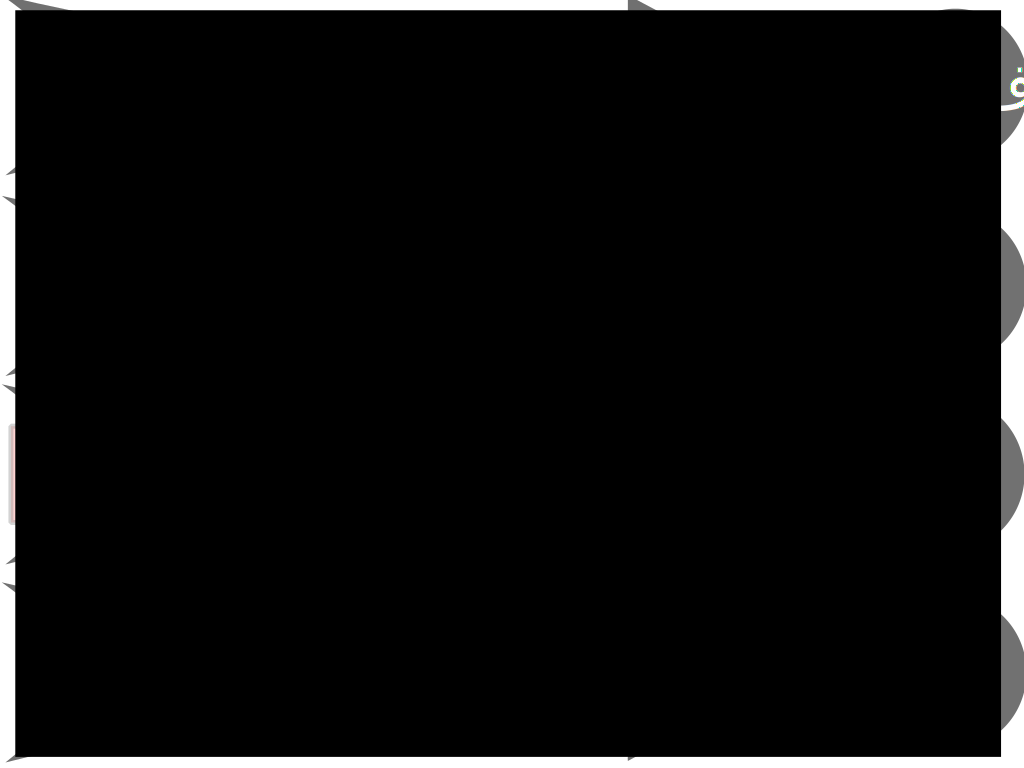
\includegraphics[width=0.75\textwidth]{image/standard/build/bamboo-workflow-objects}
\caption[فرآیند مجتمع سازی پیوسته یا \lr{CI}]{
	در این فرآيند
}
\label{image/standard/build/bamboo-workflow-objects}
\end{figure}


% Project	
% 
%     Has one, or more, plans.
%     Provides reporting (using the wallboard, for example) across all plans in the project.
%     Provides links to other applications.
% 
% Plan	
% 
%     Has a single stage, by default, but can be used to group jobs into multiple stages.
%     Processes a series of one or more stages that are run sequentially using the same repository.
%     Specifies the default repository.
%     Specifies how the build is triggered and triggering dependencies between a plan and other plans in the project.
%     Specifies notifications of build results.
%     Specifies who has permission to view and configure the plan and its jobs.
%     Provides for the definition of plan variables.
% 
% Stage	
% 
%     Has a single job, by default, but can be used to group multiple jobs.
%     Processes its jobs in parallel, on multiple agents (where available).
%     Must successfully complete all its jobs before the next stage in the plan can be processed.
%     May produce artifacts that can be made available for use by a subsequent stage.
% 
% Job	
% 
%     Processes a series of one or more tasks that are run sequentially on the same agent.
%     Controls the order in which tasks are performed.
%     Collects the requirements of individual tasks in the job, so that these requirements can be matched with agent capabilities.
%     Defines the artifacts that the build will produce.
%     Can only use artifacts produced in a previous stage.
%     Specifies any labels with which the build result or build artifacts will be tagged.
% 
% Task	
% 
%     Is a small discrete unit of work, such as source code checkout, executing a Maven goal, running a script, or parsing test results.
%     Is run sequentially within a job on a Bamboo working directory.
    
    
    
\subsection{کار مستند فنی}

ایجاد مستند فنی را می‌توان در قالب یک کار در این کارگزار در نظر گرفت. در این کار
ابتدا باید کد منبع از مخزن‌های کنترل نسخه دریافت شده و بر اساس آن مستند فنی
ایجاد شود. در نهایت مستند فنی ایجاد شده به صورت پرونده‌های فشرده ایجاد شود و به
عنوان مصنوعات در سیستم معرفی شود.


ایجاد پروژه

ایجاد نقشه

ایجاد وهله

ایجاد کار 



\subsubsection{کد منبع}

کد منبع از منبع کنترل نسخه دریافت می‌شود

\subsubsection{مستند فنی}

مستند فنی بر اساس آن ایجاد  می‌شود

\subsubsection{بسته بندی}

نتایج به دست آمده بسته بندی می شود

